% !TeX root = ../main.tex
% Add the above to each chapter to make compiling the PDF easier in some editors.

\chapter{Replication Study}\label{chapter:replication_study}

In this chapter, we first present our research questions. We then describe
our study design and setup, and both describe and evaluate the results
we obtained. We close by discussing the results in the broader context
of test suite reduction, and enumerate possible threats to validity.

\section{Research Questions}

We define four research questions, adapting three from
\cite{cruciani2019scalable} and adding one additional question on
performance in relation to a baseline algorithm.

\subparagraph{Research Question 1.1: Can the relative effectiveness in TSR be replicated on other study objects?}

We care about the size of the reduced test suite, therefore it is valuable
by how much test suites are reduced. We use the TSR metric (defined
in ~\ref{chapter:terms}) to evaluate the magnitude of the reduction.
Using the TSR is mostly useful in adequate scenarios, since in inadequate
scenarios, the size of the reduced test suite relative to the original
test suite is fixed.

\subparagraph{Research Question 1.2: Can the relative effectiveness in FDL be replicated on other study objects?}

\cite{rothermel2002empirical} finds that test suite reduction can severely
compromise fault detection capability. To test whether this is the case,
the FDL metric is used to examine the fault detection capabilities
for the algorithms given new data.

\paragraph{Research Question 2: Can the relative runtime performance of the different algorithms be replicated?}

Due to using different datasets (of both larger and smaller size), the
absolute runtimes of the different test suite reduction methods can be
expected to be different from the original runs. However, the ordering of
the methods according to runtime is expected to be the same (that is, if
algorithm $X$ was faster than algorithm $Y$ on the old data, we can expect
algorithm $X$ to also be faster than algorithm $Y$ on the new data).

\paragraph{Research Question 3: How much better than random selection are specialized algorithms?}

\cite{khan2018systematic} recommends a comparison of the examined
technique to a simple baseline. We use their recommendation (random
selection) and compare the other approaches to how well they fare against
random selection on runtime, TSR and FDL.

\section{Study Design}

We approached the research questions by collecting test case source code,
converage information and fault-detection data from projects that had
not been used in \cite{cruciani2019scalable}, and running the code from
that paper on the new data.

\paragraph{Research Question 1}

In order to answer Research Question 1, we then generated descriptive
statistics (the mean, median, and standard deviation) on the performance
measures (i.e. FDL and TSR) for the different algorithms. We then,
just as the approach in \cite{cruciani2019scalable}, first performed the
Kruskal-Wallis test for all pairs of algorithms on the same metric (with
a significance level of 5\%, as in the original paper). Algorithms for
which no statistically significant difference could be found were ranked
equally high, for algorithms with significantly different performance
we used the median FDL/TSR to determine the ranking.

We used this approach to ranking the different algorithms to ensure our
results were comparable to the results in the original paper.

The result was operationalized by assigning the algorithms letters,
with "(a)" being the signifier for the best performing algorithms,
"(b)" for the second-best, and so on (several algorithms could receive
the same ranking).

We then compared the rankings according to TSR and FDL to the ones in
\cite{cruciani2019scalable}.

\paragraph{Research Question 2}

We also computed the mean, median and standard deviation for the runtime
of the different approaches, and ranked them according to the method
described for Research Question 2.

We then compared our rankings for runtime to the ones in
\cite{cruciani2019scalable}.

\paragraph{Research Question 3}

For Research Question 3, we used the previously collected rankings
for different algorithms, and evaluated the ranking of random selection
in comparison to the other approaches presented.

\section{Study Objects}

The code bases and test suites selected for this study were small to
medium sized open-source Java projects, which we selected because tools
for generating coverage information and mutation-test data using Maven are
available and comparatively easy to use. The selected projects all used
either JUnit 4 or JUnit 5 as their testing framework, and the tool Maven
for building and testing. We used the latest version as of November 2020.

We decided to use open-source projects to make checking our generated
data easier, as well as for availability reasons.

The selected projects are both under development and in use, which makes
our results relevant to real-life systems.

The projects used, their versions and size are presented in
\autoref{tab:projects} (project and test suite size are in lines of code,
the version is the 6-digit prefix of the git commit used).

\begin{table}[htpb]
	\caption[Information about Projects Selected]{Basic Information about the selected open-source Java Projects}\label{tab:projects}
	\centering
	\begin{tabular}{l l l l l l}
		\toprule
		Project name & Version & Project size & Test-suite size & Number of tests \\
		\midrule
		assertj-core & cb2829 & 135k & 241k &3578 \\
		commons-collections & 242918 & 59k & 45k & 238 \\
		commons-lang & 6b3f25 & 51k & 40k & 181 \\
		commons-math & 649b13 & 148k & 98k & 438 \\
		jopt-simple & 5a1d72 & 1.7k & 2.7k & 145 \\
		jsoup & 89580c & 18k & 12k & 52 \\
		\bottomrule
	\end{tabular}
\end{table}

\section{Study Setup}

Testing the performance of the algorithms required three different kinds
of information: the contents of the test suites, coverage information
and fault information.

\subsection{Combining Tests Suites}

For every examined project, the test suite was converted into a format
suitable for the code from \cite{cruciani2019scalable} by replacing the
newlines from each test with spaces and concatenating the tests into one
file (the black-box file), such that every line contained one test case.

For some of the projects, test cases were excluded since they failed
during the default test run (see \autoref{tab:excluded}), with several
tests being excluded from assertj-core, one or two tests each being
excluded from the Apache commons libraries, and none from the remaining
two projects.

\begin{table}[htpb]
	\caption[Tests excluded]{Tests excluded from data gathering}\label{tab:excluded}
	\centering
	\begin{tabular}{l | p{10cm}}
		\toprule
		Project name & Test classes excluded \\
		\midrule
		assertj-core & BDDSoftAssertionsTest, SoftAssertionsTest, SoftAssertions\_overriding\_afterAssertionErrorCollected\_Test, SoftAssertionsErrorsCollectedTest, SoftAssertionsMultipleProjectsTest, SoftAssertions\_setAfterAssertionErrorCollected\_Test, AssertJMultipleFailuresError\_getMessage\_Test \\
		commons-collections & BulkTest \\
		commons-lang & FieldUtilsTest \\
		commons-math & FastMathTest, EvaluationTestValidation \\
		jopt-simple & / \\
		jsoup & / \\
		\bottomrule
	\end{tabular}
\end{table}

\subsection{Generating Coverage Information}

Since we needed information about which test covers which parts
of the program, and not just information about which parts of the
program were being covered, we used an extension to the widely used
coverage program JaCoCo, the Teamscale JaCoCo Agent (available at
\url{https://github.com/cqse/teamscale-jacoco-agent}).

Since the Teamscale JaCoCo Agent only supports line coverage, other
types of coverage had to be eschewed.

The json files created by the teamscale jacoco agent were converted
from JSON into the format used by \cite{cruciani2019scalable}: a file
containing a list of numbers in each line, with the numbers $n_1, \dots
n_i$ in line $n$ corresponding to the source lines of code in the tested
project covered by the test case at line $n$ in the black-box file.

\subsection{Collecting Fault Coverage Information}

Fault detection information was not available for the projects used, and
was therefore generated using the mutation testing framework Pitest (first
described in \cite{coles2016pit}, available at \url{http://pitest.org/}).

The generated mutation test data was converted from XML to the format
used in the code of \cite{cruciani2019scalable}: a text file containing
a list of number per line, the numbers at line $n$ corresponding to
different classes for which the test case at line $n$ in the black-box
file did find faults.

\section{Results}

To obtain the results, we used the code from \cite{cruciani2019scalable},
and applied the test suite reduction algorithms to new test data
(i.e. black-box test suite files and coverage information of 6 open source
projects) after minimal modification. These modifications were as follows:

\begin{enumerate}
\item We added a further algorithm for the random selection of test cases.
\item We fixed three bugs we found in the code, and submitted fixing changes to the the original code repository\footnote{At \url{https://github.com/ICSE19-FAST-R/FAST-R}}:
	\begin{enumerate}
	\item an off-by-one error in loading coverage information\footnote{A diff for the fix can be found at \url{https://github.com/pranomostro/thesis_code/blob/master/coverage_fix.diff}}
	\item a bug where in small test suites sometimes the candidate set would be empty\footnote{A diff for the fix of the bug can be found at \url{https://github.com/pranomostro/thesis_code/blob/master/emptycandidates_fix.diff}}
	\item a mistake where a a measured variable was not reported correctly for FAST-all\footnote{Again, a fix can be found at \url{https://github.com/pranomostro/thesis_code/blob/master/stime_fix.diff}}
	\end{enumerate}
\end{enumerate}

In the budget scenario, we considered budgets between 1\% and 30\%, with
a step increase of 1\%. We considered only line coverage, and performed
50 measurements of FDL, TSR, preparation and reduction time.

In the adequate scenario, we also considered only line coverage, and
made 50 measurements of preparation time, coverage preparation time,
and reduction time.

We did not replicate the large-scale scenario.

All measurements were performed under a Ubuntu 20.04 64-bit system,
using 6 AMD® Ryzen 5 4500u with radeon graphics processors, and 7.2
GiB of RAM available.

\subsection{Research Questions}

\paragraph{Research Question 1.1 (Can TSR findings be replicated?)}

\autoref{tab:tsr_stats} shows the descriptive statistical results
(median, standard deviation and ordering for the Kruskal-Wallis test)
in the adequate case, and \autoref{fig:tsr_box} shows boxplots for
TSR for the different algorithms.

For Java programs with statement coverage in the adequate case,
\cite{cruciani2019scalable} order the different methods of test suite
reduction according to TSR. Their results mostly agree with ours: They
rank GA highest, then FAST++ and FAST-pw, then FAST-CS, FAST-all below
that, and the ART family lowest; we also rank GA highest, followed by
FAST++, then FAST-CS and FAST-pw at the same level, then FAST-all, and
the ART family last (on par with random selection). However, the median
test suite reduction they report for these methods is much lower than what
we observe (at least for the java programs): even GA only achives a TSR
of 12.30, while in our experiment GA achieves a TSR of over 40. However,
their results with C programs are more stark than ours, achieving a TSR
of more than 90 for GA or FAST++.

%CANDO: Use Borda-count to determine the amount of agreement in these
%rankings?

Our data shows higher variance in TSR performance on all algorithms.

\begin{table}[htpb]
	\caption[TSR statistical results, adequate]{Different variables relating to TSR (mdn is the median, $\sigma$ being the standard deviation, and $\delta$ being the ranking in the Kruskal-Wallis test)}\label{tab:tsr_stats}
	\centering
	\begin{tabular}{| l | l | l | l | l |}
	\midrule
	Approach & $\mu$ & mdn & $\sigma$ & $\delta$ \\
	\midrule
	ART-D & 18.421 & 17.351 & 8.997 & (e) \\
	ART-F & 0.945 & 0.228 & 1.654 & (f) \\
	FAST++ & 36.116 & 33.811 & 13.581 & (b) \\
	FAST-all & 21.414 & 18.264 & 8.536 & (d) \\
	FAST-CS & 33.683 & 31.893 & 12.064 & (c) \\
	FAST-pw & 33.258 & 32.718 & 11.458 & (c) \\
	GA & 40.599 & 39.124 & 14.922 & (a) \\
	RS & 0.947 & 0.420 & 1.491 & (f) \\
	\bottomrule
	\end{tabular}
\end{table}

\begin{figure}[h]
\caption[TSR boxplots, adequate]{Boxplots for TSR for different algorithms in the adequate case}\label{fig:tsr_box}
\centering
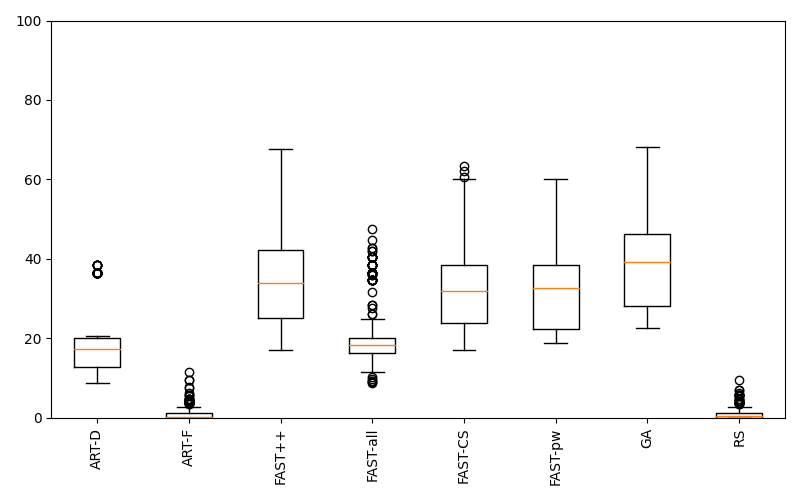
\includegraphics[scale=0.7]{figures/tsrs.png}
\end{figure}

\paragraph{Research Question 1.2 (CAN FDL findings be replicated?)}

\autoref{tab:fdl_stats} shows the descriptive statistics (mean, median,
standard deviation, and ordering according to the Kruskal-Wallis test)
for the FDL of different algorithms in both the budget and adequate case,
and \autoref{fig:fdl_box} shows boxplots for FDL for different algorithms.

We compare our findings to FDL performance on statement-covered C
program data, since the fault information for the java programs used
in \cite{cruciani2019scalable} is very sparse (1-3 faults per program),
while fault information is much richer for the C programs.

In the budget scenario, we could not detect strong differences in
performance in FDL. All algorithms score equally, with the exception
of GA dominating every other algorithm and RS being dominated by every
other algorithm. Here, again, \cite{cruciani2019scalable} come to very
similar conclusions: They find that GA is statistically significantly
better than all other algorithms, which are in turn approximately equally
effective at detecting faults.

Here, we also find that the standard deviations in FDL for our data
is higher than the ones in \cite{cruciani2019scalable}. Similar to
their findings, we see no strong difference in variance for different
algorithms.

In the adequate case, our data ranks the algorithms into just two
categories: The better-performing category contains algorithms
from the ART family, FAST++ and FAST-CS, while the rest of
the approaches is sorted into the bucket of worse-performing
approaches. \cite{cruciani2019scalable} agrees that the ART family
is best-performing, but find that FAST-all is second-best, GA being
third-best, and FAST-CS, FAST-pw and FAST++ coming last. At the moment,
we don't have a hypothesis about why this might be the case. It seems
relevant, however, that the median fault detection loss for data was 0 for
all algorithms (the mean fault detection loss being non-zero, however),
just as the ART family and FAST-all in \cite{cruciani2019scalable}.
Perhaps this is caused by single tests both having large coverage and
detecting a majority of faults.

This hypothesis is further supported by the observation that the variance
in performance on all algorithms is much lower than in the original paper,
for all algorithms.

\begin{table}[htpb]
	\caption[FDL statistical results]{Different variables relating to FDL ($\mu$ being the mean, mdn the median, $\sigma$ the standard deviation, and $\delta$ the ranking in the Kruskal-Wallis test)}\label{tab:fdl_stats}
	\centering
	\begin{tabular}{| c | c | c}
	\midrule
	Budget & Adequate \\
	\midrule
	{\begin{tabular}{l | l | l | l | l}
		Approach & $\mu$ & mdn & $\sigma$ & $\delta$ \\
		\midrule
		ART-D & 76.414 & 94.75 & 34.502 & (b) \\
		ART-F & 77.72 & 95.04 & 35.684 & (b) \\
		FAST++ & 76.49 & 94.05 & 35.662 & (b) \\
		FAST-all & 74.78 & 92.19 & 35.269 & (b) \\
		FAST-CS & 76.19 & 93.39 & 35.493 & (b) \\
		FAST-pw & 71.63 & 93.82 & 35.665 & (b) \\
		GA & 62.53 & 70.45 & 33.367 & (a) \\
		RS & 93.43 & 97.46 & 9.305 & (c) \\
	\end{tabular}} &
	{ \begin{tabular}{l | l | l | l | l}
		Approach & $\mu$ & mdn & $\sigma$ & $\delta$ \\
		\midrule
		ART-D & 0.129 & 0.0 & 0.702 & (a) \\
		ART-F & 0.057 & 0.0 & 0.679 & (a) \\
		FAST++ & 1.122 & 0.0 & 2.172 & (a) \\
		FAST-all & 0.155 & 0.0 & 0.331 & (b) \\
		FAST-CS & 1.144 & 0.0 & 2.367 & (a) \\
		FAST-pw & 0.792 & 0.0 & 1.131 & (b) \\
		GA & 1.432 & 0.0 & 2.444 & (b) \\
		RS & 0.058 & 0.0 & 0.679 & (b) \\
	\end{tabular}} \\
	\bottomrule
	\end{tabular}
\end{table}

\begin{figure}[h]
\caption[FDL boxplots]{Boxplots for FDL for different algorithms}\label{fig:fdl_box}
\centering
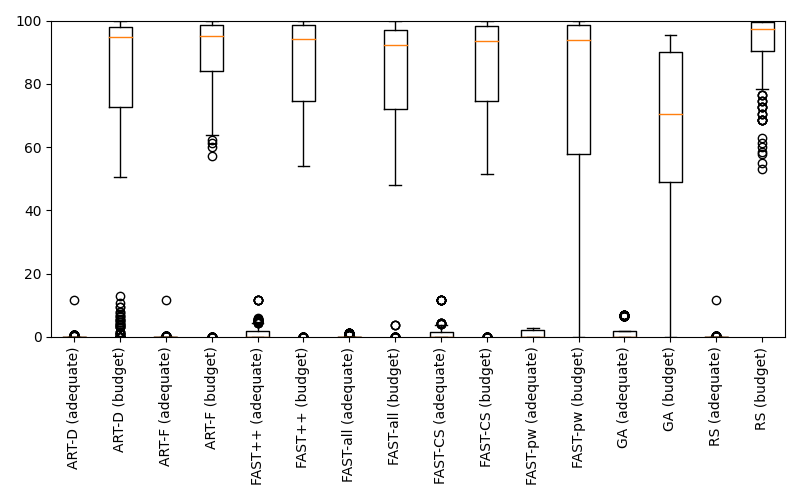
\includegraphics[scale=0.7]{figures/fdls.png}
\end{figure}

We include the mean in the descriptive statistics to illustrate that
while the median adequate reduction has no fault detection loss, it can
nonetheless still occur.

\paragraph{Research Question 2 (Can total runtime performance findings be replicated?)}

\autoref{tab:total_stats} lists statistics for the total reduction times
in seconds ("total" including the time for loading the coverage files,
the time for processing the black-box test files, and the reduction
time). The table lists both the median and the mean of the total time,
since especially in the adequate case there are big differences in these
measurements (e.g. in the case of ART-D, where the mean reduction time is
more than two orders of magnitude greater than the median reduction time).

Comparing the budget scenario to the statement-coverage based budget
(we remove function and branch-coverage based approaches) scenario in
\cite{cruciani2019scalable}, one can observe striking differences. While
GA performs best in our measurements, the original paper ranks it
in the middle (although, in the function-based coverage test, their
measurements agree with ours). The approaches from the FAST family perform
rather mediocre, receiving ranks (d) (FAST++ and and FAST-CS) and (e)
(FAST-all and FAST-pw), while in the original measurements, FAST++
is ranked second-best, followed by FAST-CS, and FAST-all and FAST-pw
being ranked lowest. Algorithms from the ART family receive relatively
high rankings in our measurements ((b) and (c)), while in the original
measurements, they also perform mediocre (around as well as GA).

In the adequate scenario, we also only examine the statement-coverage
based measurements from the original paper. Our results rank RS highest,
followed by GA, while GA receives only rank (c) in the original results.
From the FAST family, FAST++ and FAST-CS rank just below GA, while
in the original results, they come out as clear winners. FAST-pw and
FAST-all rank are ranked lowest in our results, even below the ART family,
while in the original results, ART algorithms are clearly ranked lowest.
We suspect that this result is due to the difference in medians between
the datasets we used and the original dataset: The dataset we used
contained several relatively small test suites, and a relatively big
outlier, while the test suites in the original paper were more similar
in size. That leads to comparatively small medians (and comparatively
large means) in total runtime for our data (as can be seen in the greater
standard deviations) on the ART algorithms. Since the Kruskal-Wallis
test we and \cite{cruciani2019scalable} use only considers medians for
ordering, the outliers do not influence the final ordering.

\begin{table}[htpb]
	\caption[Runtime performance statistical results]{Different variables relating to total runtime in seconds ($\mu$ being the mean, mdn the median, $\sigma$ the standard deviation, and $\delta$ the ranking in the Kruskal-Wallis test)}\label{tab:total_stats}
	\centering
	\begin{tabular}{| c | c | c}
	\midrule
	Budget & Adequate \\
	\midrule
	{\begin{tabular}{l | l | l | l | l}
		Approach & $\mu$ & mdn & $\sigma$ & $\delta$ \\
		\midrule
		ART-D & 0.81 & 0.975 & 0.318 & (b) \\
		ART-F & 0.919 & 0.982 & 0.133 & (c) \\
		FAST++ & 1.064 & 1.156 & 0.545 & (d) \\
		FAST-all & 7.005 & 3.567 & 8.425 & (e) \\
		FAST-CS & 1.034 & 1.152 & 0.506 & (d) \\
		FAST-pw & 7.025 & 3.582 & 8.473 & (e) \\
		GA & 0.974 & 0.968 & 0.632 & (a) \\
		RS & 0.95 & 0.982 & 0.087 & (c) \\
	\end{tabular}} &
	{ \begin{tabular}{l | l | l | l | l}
		Approach & $\mu$ & mdn & $\sigma$ & $\delta$ \\
		\midrule
		ART-D & 58.232 & 0.475 & 127.311 & (e) \\
		ART-F & 158.892 & 1.926 & 341.625 & (f) \\
		FAST++ & 1.792 & 0.329 & 3.254 & (c) \\
		FAST-all & 6.345 & 2.622 & 8.494 & (f) \\
		FAST-CS & 2.232 & 0.334 & 4.053 & (d) \\
		FAST-pw & 8.224 & 2.736 & 12.206 & (g) \\
		GA & 4.286 & 0.147 & 8.725 & (b) \\
		RS & 0.965 & 0.143 & 1.535 & (a) \\
	\end{tabular}} \\
	\bottomrule
	\end{tabular}
\end{table}

%CANDO: Compare to just reduction times as well?

\paragraph{Research Question 3 (How well do algorithms perform against a random baseline?)}

In short, the answer is that they perform better on performance metrics,
while being slower. \autoref{tab:tsr_stats} shows that RS ranks lowest
on TSR (together with ART-F). Similarly, \autoref{tab:fdl_stats} ranks
RS lowest on FDL in the budget and adequate case (although in the latter
case, RS can not be shown to be statistically significantly worse than
three other algorithms). We also found that RS performs surprisingly
badly in terms of runtime performance (see \autoref{tab:total_stats}) in
the budget case, ranking third, despite being the conceptually simplest
algorithm we examined. However, in the adequate case, it ranks best.

\section{Discussion}

In general, we find that our results largely replicate the
results in \cite{cruciani2019scalable}. On TSR and FDL, we (and
\cite{cruciani2019scalable}) rank GA very high, often first, usually
followed by FAST++ and FAST-CS, then FAST-pw and FAST-all, then the
ART algorithms and finally RS. With regards to FDL, we often can't
statistically significantly differentiate the algorithms in performance,
similar to the original paper.

Our results in runtime performance differ from the original results,
though, disagreeing both in the adequate and the budget case. We
hypothesize that this is due to different distributions in the sizes
of the test suites tested on, with the test suites we used being both
smaller and larger than the test suites used in the original paper, which
makes the median of runtimes less useful at determining the relative
performance of algorithms.

We cautiously conclude that for test suites of the sizes we have examined,
the GA algorithm makes a good trade-off between test suite reduction,
fault detection loss and runtime performance, if coverage information
is available.

\section{Threats to Validity}

Although we attempted to prevent it, the results we obtained might suffer
from threats to validity.

\subsection{Construct Validity}

Construct validity considers whether the methods are adequate to answer
the research questions posed. As in the original paper, we used FDL
and TSR as standard metrics, and reported the mean, median and standard
deviation of the data as standard statistical properties of the generated
data. We used faults generated by mutation testing software instead of
real faults, which might be dissimilar from real faults. However, it
has been argued that mutation faults are similar to real-world faults
(\cite{budd1980mutation}, and programmers of mutation-testing software
try to make the faults introduced as realistic as possible.

To prevent bugs from our code and the code by \cite{cruciani2019scalable}
introducing incorrect results, we checked the code using a small,
transparently understandable test project. We then manually verified
that this project was handled correctly. This led to finding one of
the bugs in the original code by \cite{cruciani2019scalable}.

Due to restrictions on availability, we used line coverage instead of
statement coverage. Since the original study mostly examined statement
coverage, there might be problems in comparing the results of the two
studies (such as statements spanning multiple lines, or several statements
in one line). However, we claim that in practice, statement coverage
and line coverage are similar in terms of granularity.  For example,
both \cite{an2018comparing} and \cite{yang2009survey} treat statement
and line coverage as equivalent.

To enable verification of our methods, we published the code for this
replication at \url{https://github.com/pranomostro/thesis_code}.

\subsection{Internal Validity}

The results we obtained might not be due to actual differences in
the performance of the different methods, but due to other factors,
such as the usage of the computer used for gathering data for other
purposes during that time. To migitate these effects, we performed every
measurement 50 times, and abstained from using the computer during the
time of gathering data.

%CANDO: add point about very different runtimes on different
%projects, maybe attach distribution images?

\subsection{External Validity}

The projects we selected are all small to medium-sized projects,
and therefore the results we obtained might not generalize to
large-scale software systems. While one of the projects we obtained
test data from (assertj-core) was larger than the projects examined in
\cite{cruciani2019scalable}, it was not analyzed separately from the
other data. However, since the projects we used were of similar size
as the ones in \cite{cruciani2019scalable}, and our interest was to
replicate their findings, we regard this consideration as less relevant.
